\documentclass[12pt]{article}
\usepackage{amssymb,mathrsfs, amsmath,amsfonts}
\usepackage{mathtools}
\usepackage{graphicx}
\usepackage{enumitem}
\usepackage{braket}
\graphicspath{ {./ps1-assets/}{./exercises/ps1-assets/} }

\title{Problem Set 1}
\author{CSE 468}
\date{May 2021}

\begin{document}

\maketitle

\noindent \textbf{Note:} Many of these problems use https://lab.quantumflytrap.com/lab.

\begin{enumerate}[font=\bfseries]
    \item Create the following setup in your own workspace.\\
    \[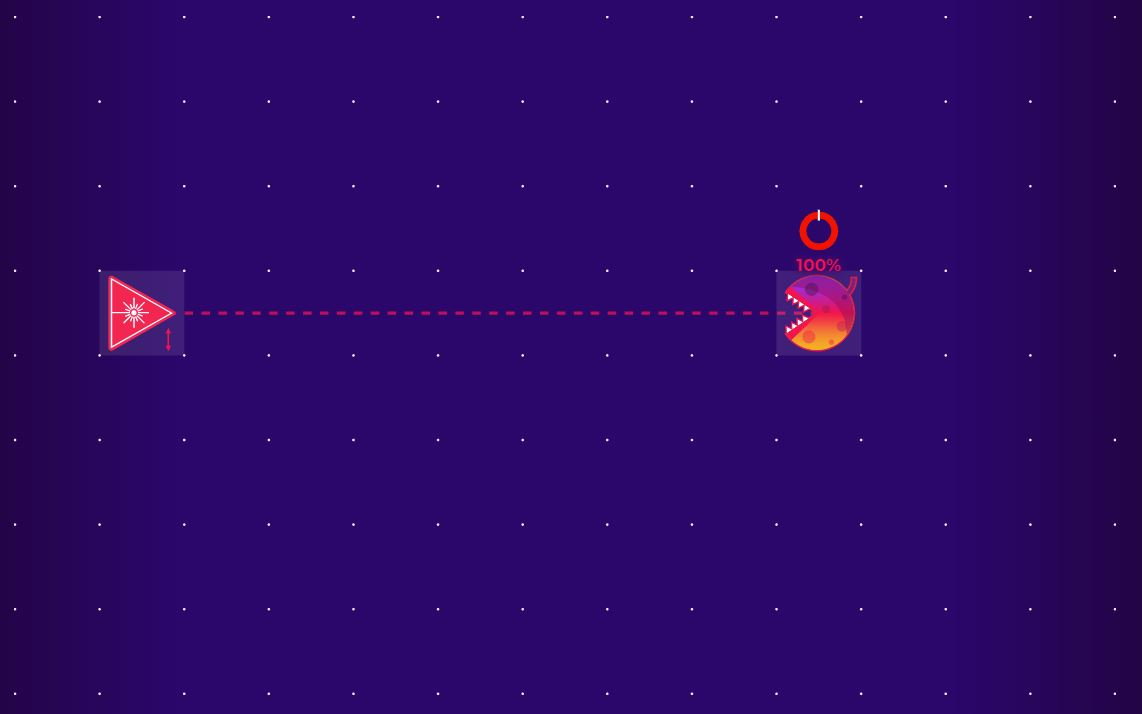
\includegraphics[scale=0.4]{easyFilter}\]
    \begin{enumerate}
        \item Using only polarizing filters create a configuration such that the detector only detects 6.25$\%$ of the initial photons. Please upload a picture of your configuration.
        \item Describe a general strategy using only polarizing filters that causes the detector to detect only $n\%$ of the initial photons. You may assume $n \leq 100$ and $n = \frac{100}{2^k}$ with $k\in\mathbb{Z}^+$.
        \item There is only one path in this configuration so we can instead use state to represent the polarization of the photons. Let $\ket{0} = \begin{pmatrix}1 \\ 0 \end{pmatrix}$ represent photons completely oriented in the horizontal direction. Similarly, let $\ket{1} = \begin{pmatrix}0 \\ 1 \end{pmatrix}$ represent photons completely oriented in the vertical direction. Note we can characterize any state of these bases by a single parameter $\theta$ as follows $\ket{\psi} = \cos{\theta}\ket{0} + \sin{\theta}\ket{1}$. Using this notation describe the matrix that represents a polarizing filter oriented in the vertical direction.
        \item Given some state $\ket{\psi}$, what is the chance, in terms of $\theta$, that the photon will pass through a vertically oriented filter?
        \item Give the matrix that describes a general polarizing filter oriented $\theta$ degrees from the origin.
        \item Using the above notation, describe the state of your system at each step.
        \item Does applying a vertical filter, then a horizontal filter, and then a 45 degree filter produce the same result as applying a vertical filter, then a 45 degree filter, and then a horizontal filter? Why or why not?
    \end{enumerate}
    \item Create the following setup in your own workspace.
    \[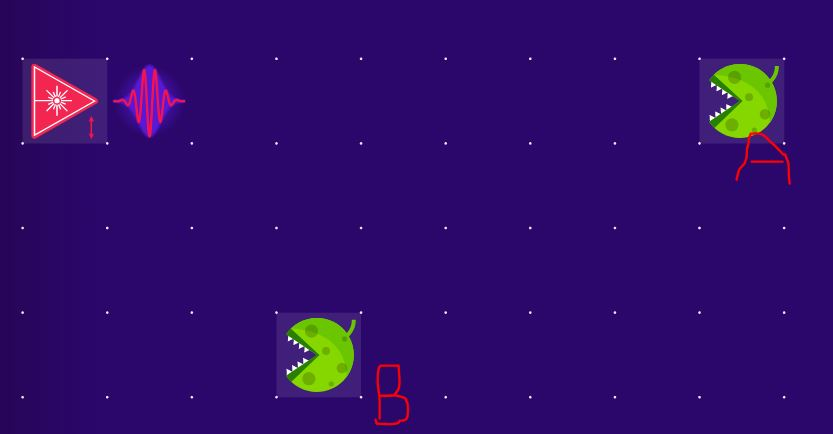
\includegraphics[scale=0.6]{beamSplit}\]
    Read about the polarizing beam splitter and understand how it behaves with various inputs.
    \begin{enumerate}
        \item Using only polarizing beam splitters and polarizing filters, create a configuration such that the probability of measuring a photon at Receiver A and the probability of measuring a photon at Receiver B are both greater than zero.
        \item What is the maximum possible combined probability of a photon arriving at Receiver A or Receiver B? Why?
        \item Give the matrix that describes the polarizing beam splitter. 
        \item Using your result from (c) describe the state of your system at each step.
    \end{enumerate}
    \item Recreate the initial configuration of Question 2. Read about the sugar solution tool.
    \begin{enumerate}
        \item Using only sugar solutions and polarizing beam splitters create a configuration such that the probability of measuring a photon at Receiver A and the probability of measuring a photon at Receiver B are both greater than zero.
        \item What is the maximum possible combined probability of a photon arriving at Receiver A or Receiver B? Why?
        \item Give the matrix that describes the sugar solution.
        \item Using your result from (c) describe the state of your system at each step.
    \end{enumerate}
    \item Your good friend, Niels Bohr, needs your help with a quantum experiment. Bohr has set up a complicated quantum system to make some computation. The problem is Bohr doesn’t know how to figure out what the actual output of his system is. Your task is, given Bohr’s system, describe how to make a measurement of either 0 or 1. For this question, a photon from the source we say begins in state 0 and is 0 degree relative to the source. A photon rotated 90 degrees from the source we say is in state 1. Assume Bohr’s result is either completely 0 or completely 1. 
    \item Go to the experimental setups section (in the top left menu). Choose the quantum coin flip experiment. Click the detections mode in the bottom left and then click Play x100 and click run. This will run the experiment 100 times, keeping track of the number of photons that arrive at each receiver. 
    \begin{enumerate}
        \item How many counts should we expect to see in each receiver? Run the experiment and report your results.
        \item Do your results match your predictions? Why or why not?
    \end{enumerate}
    \item Consider the setup below.
    \[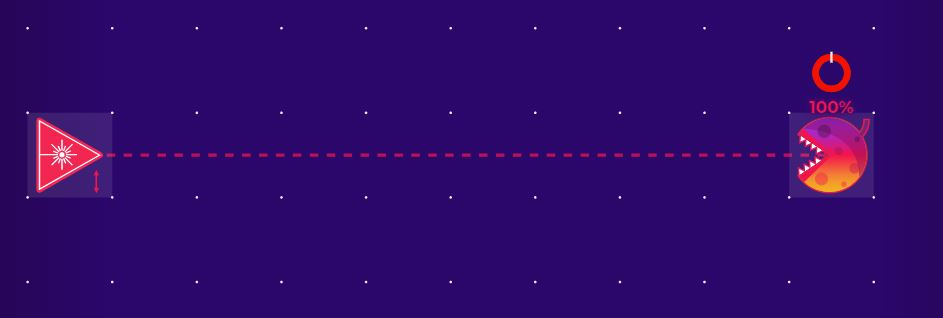
\includegraphics[scale=0.6]{rotate10}\]
    This website only allows us to rotate polarizing filters in increments of 45 degrees. Let's imagine that we were able to rotate polarizing filters in increments of 10 degrees.
    \begin{enumerate}
        \item How many polarizing filters could we place between the photon source and receiver and still expect to see at least 50\% of the initial photons in the receiver?
    \end{enumerate}
\end{enumerate}



\end{document}
